\section{Method}
\label{sec:method}
Bug bounty programs work on the premises that humans are efficient at searching and finding vulnerabilities, in particular when large pools of security researchers with a variety of skills can be mobilized for the task. It is in the interest of the organization launching a bounty program to {\it exhaust} vulnerabilities, or to reduce the probability of finding additional vulnerabilities to a residual level. In addition, incentives must be carefully set. Here, we investigate the interplay between the vulnerability exhaustion process, and the cumulative bounty prizes distributed to security researchers within and across bounty programs. When a bug bounty program starts, it attracts a number of security researchers, who in turn submit bugs. Subsequent bug discoveries get increasingly difficult \cite{brady1999murphy}, and program managers must reward vulnerabilities accordingly to keep security researchers onboard (or to attract new ones according to the current level of difficulty). %As we will see, keeping security researchers onboard, at least those who have already heavily contributed, is critical to the exhaustion process. 

Starting from an initial probability of discovering the first vulnerability $P(k=0) = 1$, we assume that the probability to find a second (and subsequent) vulnerabilities, is a fraction of the former probability: $P(k+1) = \beta * P(k)$ with $\beta$ a constant strictly smaller than, yet usually close to $1$. 
The probability that no more discovery will be made after $k$ steps is given by $P(k) = \beta^{k} (1-\beta)$. Conversely, starting from the initial reward $R_0 = R(k=0)$, the subsequent reward $R_1 = \Lambda_1 \cdot R_0$, and further additional reward $ R_2 = \Lambda_2 \Lambda_1 \cdot R_{0}$. After $n$ steps, the total reward is the sum of all past rewards: 

\begin{equation}
R_{n} = R_{0} \sum_{k=1}^{n} \Lambda_1 ... \Lambda_k.
\end{equation}

Thus, $R_{n}$ is the recurrence solution of the 
Kesten map ($R_{n} = \Lambda_n R_{n-1} +R_0$)
\cite{kesten1973random,sornette1997convergent}:  As soon as amplification occurs (technically, 
some of the factors $\Lambda_k$ are larger than $1$), the distribution
of rewards is a power law, whose exponent $\mu$ is a function of $\beta$
and of the distribution of the factors $\Lambda_k$. In the case where
all factors are equal to $\Lambda$, this model predicts three possible regimes for the distribution of rewards (for a given program): thinner than exponential for $\Lambda < 1$, exponential for $\Lambda = 1$, and power law for $\Lambda > 1$ with exponent $\mu = |\ln \beta|/ \ln \Lambda$ (see Appendix). The expected utility of vulnerability discovery is thus given by,

\begin{equation}
\label{ }
U_k = P_k \times R_k,
\end{equation}

\noindent with both $P_k$ and $R_k$ random variables respectively determined by $\beta$ and $\Lambda$. The nature of $U$ is reminiscent of the St. Petersburg paradox (or St. Petersburg lottery), proposed first by the Swiss Mathematician Nicolas Bernoulli in 1713, and later formalized by his brother Daniel in 1738 \cite{bernoulli1954exposition}. The St. Petersburg paradox states the problem of decision-making when both the probability and the reward are diverging, yet the expected utility increases (in the simplest case, proposed by Bernouilli $U_n = \sum_{k=0}^{n} U_k = n$) \cite{bernoulli1954exposition}. $U(k)$ therefore determines the incentive structure for security researchers, given that the bounty program manager can tune $R_0$ and in some cases, the manager can also tune $\Lambda$. However, in general rules are set upfront and shall not be changed in the course of the bounty program. Changing rules of game is risky as it may undermine trust in the program. Here, we assume the bounty program managers don't tune their reward policy after the bug bounty program has started. Because of learning effects, which we will detail below, the crowd initially involved (for $k$ small) also predicts long-term activity, in particular for the discovery of highly ranked vulnerabilities {\bf (as a result of learning /expertise effects?)}. In principle, the manager could set $R_0$ to influence $P_0$ and indirectly $P$. Mapping the discovery rank $k$ into the rate of discovery may also allow consider discounting aspects in presence of competing opportunities \cite{} and inter-time choices dependencies \cite{}.\\

A new bounty program is launched at a Poisson rate, approximately every 2 months, and each launch brings its windfall effect, leaving the researcher with the choice to either keeping digging increasingly harder vulnerabilities (rare but with higher reward), or turning to the low hanging fruits (frequent but with low reward) of a new program. We shall therefore verify whether newly launched programs actually influence security researchers.







%The propensity for security researchers to keep searching for vulnerabilities is conditioned by the trend of $U(k)$: if $U \rightarrow 0$ when $k \rightarrow \infty$, then it's likely that they will leave the program (it's a bit sketchy here). If do not consider the costs (i.e., effort spent on finding the $k^{th}$ bug, which we cannot measure here (see next subsection on timing effects), but which is indirectly captured by $P(k)$), then in the presence of a variety of programs at different stages of their life (i.e., at different values of $k$), the security researcher is left with comparing utility between programs.









%\begin{figure}
%\begin{center}
%%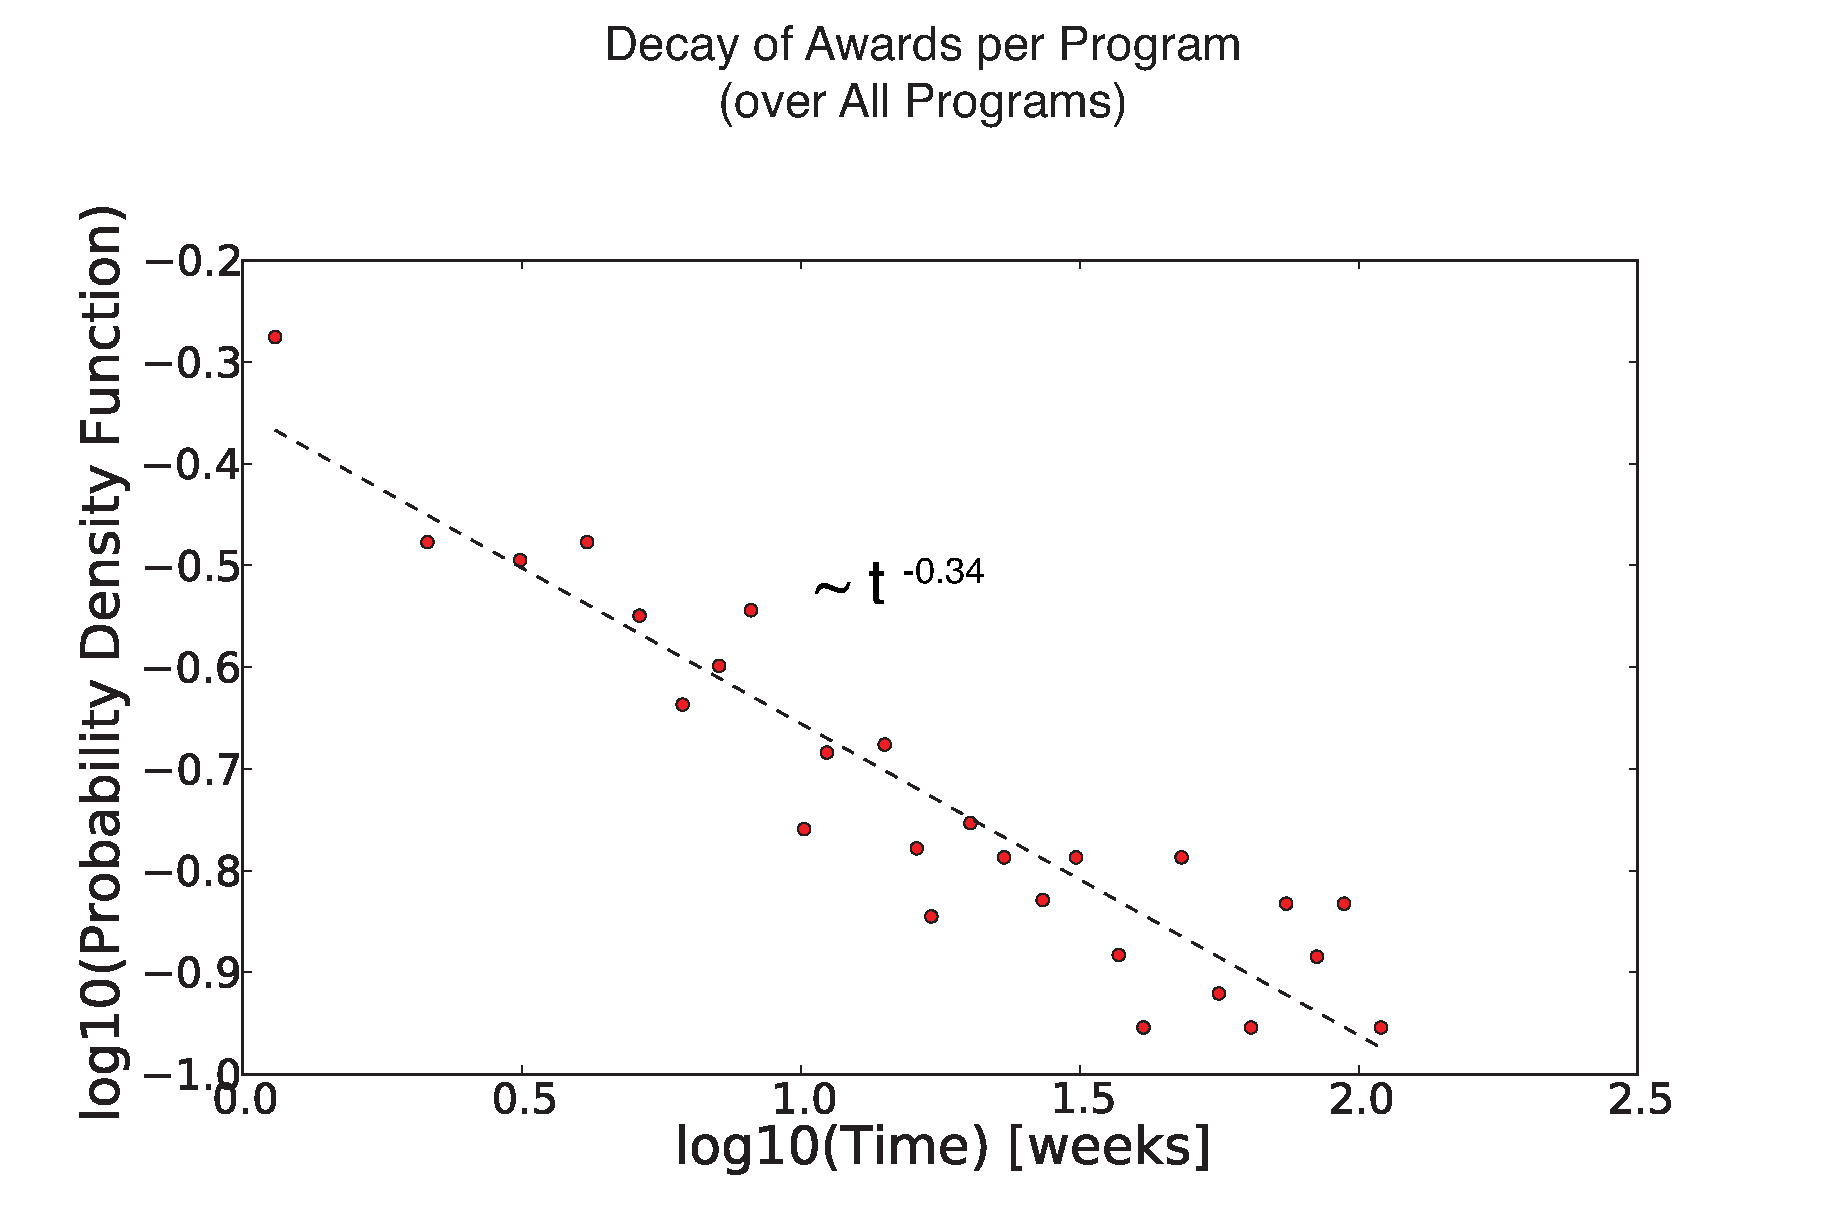
\includegraphics[width=10cm]{figures/decay.eps}
%\caption{Distribution of discovery waiting time between ranks $\rightarrow$ the hope is to find that time increases as $k \rightarrow \infty$.}
%\label{fig:decay}
%\end{center}
%\end{figure}





%The incentive mechanism is then completely driven by the probability of discovery of the $k+1$ vulnerability given that $k$ bugs have already been discovered on the one hand, and by the expected reward for the $k+1$ discovery on the other hand. When the probability of finding a bug decreases fast while the reward for a new bug increases fast, in such a way that the product $f_k \times R_k$ remains constant, then the expected value of the game increases linearly as $k \rightarrow \infty$. This problem is reminiscent 


%When a bug bounty program (by an organization) is launched immediate vulnerabilities are found by security researchers and rewarded by organizations. The cost of finding a new vulnerability increases as more discoveries occur, and thus, incentives should be set accordingly to keep onboard security researchers, or at least, the best researchers who have the capabilities to find increasingly subtle problems. 



%Searching for bugs in software is an attrition process: When the search starts, obvious bugs are found first. Subsequent bug discoveries get increasingly difficult. When a bug bounty program (by an organization) is launched immediate vulnerabilities are found by security researchers and rewarded by organizations. The cost of finding a new vulnerability increases as more discoveries occur, and thus, incentives should be set accordingly to keep onboard security researchers, or at least, the best researchers who have the capabilities to find increasingly subtle problems. 
%
%{\bf aim 1:} understand the evolution of expected utility of security researchers as an increasing amount of vulnerabilities get discovered for a given program. And how the incentive mechanism varies from one program to another\\
%
%{\bf aim 2:} understand how bug bounties compete with each others? Each time, a new bug bounty program is launched, a new set of opportunities arises, and security researchers must make a choice (though not a binary choice) between digging further in an existing program (with lower probability to find a vulnerability, but presumably with higher utility) or turning to a new program (with higher probability to find a vulnerability, but presumably with lower utility).
%
%{\bf aim3: } What can we say about the whole eco-system?


